%%%%%%%%%%%%%%%%%%%%%%%%%%%%%%%%%%%%%%%%%
% Stylish Article
% LaTeX Template
% Version 2.0 (13/4/14)
%
% This template has been downloaded from:
% http://www.LaTeXTemplates.com
%
% Original author:
% Mathias Legrand (legrand.mathias@gmail.com)
%
% License:
% CC BY-NC-SA 3.0 (http://creativecommons.org/licenses/by-nc-sa/3.0/)
%
%%%%%%%%%%%%%%%%%%%%%%%%%%%%%%%%%%%%%%%%%

%----------------------------------------------------------------------------------------
%	PACKAGES AND OTHER DOCUMENT CONFIGURATIONS
%----------------------------------------------------------------------------------------

\documentclass[fleqn,10pt]{SelfArx_063318} % Document font size and equations flushed left
 
%----------------------------------------------------------------------------------------
%	COLUMNS
%----------------------------------------------------------------------------------------

\setlength{\columnsep}{0.55cm} % Distance between the two columns of text
\setlength{\fboxrule}{0.75pt} % Width of the border around the abstract

%----------------------------------------------------------------------------------------
%	COLORS
%----------------------------------------------------------------------------------------

\definecolor{color1}{RGB}{0,0,90} % Color of the article title and sections
\definecolor{color2}{RGB}{0,20,20} % Color of the boxes behind the abstract and headings

%----------------------------------------------------------------------------------------
%	HYPERLINKS
%----------------------------------------------------------------------------------------

\usepackage{hyperref} % Required for hyperlinks
\hypersetup{hidelinks,colorlinks,breaklinks=true,urlcolor=color2,citecolor=color1,linkcolor=color1,bookmarksopen=false,pdftitle={Title},pdfauthor={Author}}

%----------------------------------------------------------------------------------------
%	ARTICLE INFORMATION
%----------------------------------------------------------------------------------------

\JournalInfo{Evaluación Final Biomat} % Journal information
\Archive{Actualizado 14-06-2023} % Additional notes (e.g. copyright, DOI, review/research article)

\PaperTitle{Análisis de Heterogeneidad Espacial en Modelos Epidemiológicos}

\Authors{Luis Ernesto Ibarra Vázquez\textsuperscript{1}}
\affiliation{\textsuperscript{1}\textit{Centro de Neurociencias de Cuba, La Habana, Cuba, luisernesto.ibarra@cneuro.edu.cu, luise98cu@gmail.com}} % Author affiliation
%\affiliation{*\textbf{Autor para Correspondencia, Corresponding Author}} % Corresponding author

\Keywords{Biomatemática, heterogeniedad espacial, modelado matemático} % Keywords - if you don't want any simply remove all the text between the curly brackets

%----------------------------------------------------------------------------------------
%	ABSTRACT
%----------------------------------------------------------------------------------------

\Abstract{
Este reporte presenta una introducción a la Biomatemática, un campo interdisciplinario que aplica 
métodos matemáticos y computacionales para modelar sistemas biológicos complejos. Se explica la importancia 
de representar la heterogeneidad espacial en modelos ecológicos y epidemiológicos, lo cual permite una 
comprensión más profunda de procesos del mundo real. Se presenta el modelo epidemiológico SIR y se discuten 
sus limitaciones al asumir homogeneidad espacial. Luego, se propone un esquema de modelado que incorpora 
heterogeneidad mediante la definición de metapoblaciones, esquemas de separación, y reglas de intercambio. 
Se muestran ejemplos de modelos espacialmente explícitos y sus aplicaciones para el estudio de COVID-19. El 
reporte brinda las bases para comenzar a estudiar y aplicar técnicas de modelado espacial en diversas áreas de 
la biología.
}

%----------------------------------------------------------------------------------------

\begin{document}

\flushbottom % Makes all text pages the same height

\maketitle % Print the title and abstract box

%\tableofcontents % Print the contents section

\thispagestyle{empty} % Removes page numbering from the first page

%----------------------------------------------------------------------------------------
%	ARTICLE CONTENTS
%----------------------------------------------------------------------------------------

\section*{Reporte de investigación} % The \section*{} command stops section numbering
\section{Introducción}

La Biomatemática es un campo interdisciplinario que aplica principios matemáticos y computacionales para modelar y
analizar sistemas biológicos complejos. Esta integración de biología, estadística y modelado matemático busca
entender y hacer predicciones sobre organismos vivos y sus interacciones. Mediante el desarrollo de modelos
cuantitativos, la Biomatemática ayuda a revelar relaciones y patrones difíciles de detectar solo con experimentación
biológica.

La heterogeneidad espacial es un fenómeno común en sistemas biológicos y ecológicos. Se refiere a la variación en las
propiedades de un sistema a través del espacio, como diferencias en la densidad de población, distribución de recursos,
o condiciones ambientales. Modelar matemáticamente esta heterogeneidad espacial puede proporcionar información valiosa
sobre los procesos subyacentes y la dinámica de estos sistemas.

La habilidad de representar adecuadamente la heterogeneidad espacial puede mejorar significativamente la
comprensión de patrones y procesos en ecología, epidemiología y evolución. Los modelos desarrollados en este campo
tendrán aplicaciones para problemas importantes como la propagación de enfermedades infecciosas y la dinámica de
metapoblaciones.

En el reporte se mencionan algunas de las maneras que existen en la literatura para el modelado y análisis de
modelos y variables que toman en cuenta la heterogeneidad espacial. Se mencionan pasos a tener en cuenta para la
confección de este tipo de modelos.

\section{Desarrollo}

\subsection{Modelo SIR clásico}

El modelo SIR se utiliza para describir la propagación de enfermedades infecciosas en una población.
Proporciona una representación matemática de cómo la enfermedad se propaga a lo largo del tiempo y cómo
evoluciona la cantidad de personas en cada categoría (susceptibles (S), infectados (I) y recuperados (R)).

\textbf{Ecuaciones del modelo:}

Las ecuaciones diferenciales que rigen el modelo SIR son las siguientes:
\begin{equation*}
    \frac{dS}{dt} = -\beta \cdot S \cdot I
\end{equation*}
\begin{equation*}
    \frac{dI}{dt} = \beta \cdot S \cdot I - \gamma \cdot I
\end{equation*}
\begin{equation*}
    \frac{dR}{dt} = \gamma \cdot I
\end{equation*}

Donde:
\begin{itemize}
    \item $S$ es la cantidad de personas susceptibles.
    \item $I$ es la cantidad de personas infectadas.
    \item $R$ es la cantidad de personas recuperadas.
    \item $\beta$ es la tasa de transmisión de la enfermedad.
    \item $\gamma$ es la tasa de recuperación de la enfermedad.
\end{itemize}

Estas ecuaciones describen cómo cambian las cantidades de susceptibles, infectados y recuperados en función del tiempo.
El término $-\beta \cdot S \cdot I$ en la ecuación de $\frac{dS}{dt}$ representa la tasa de personas susceptibles que
se infectan, mientras que el término $\gamma \cdot I$ en la ecuación de $\frac{dR}{dt}$ representa la tasa de personas
infectadas que se recuperan. El término $\beta \cdot S \cdot I$ en la ecuación de $\frac{dI}{dt}$ representa la tasa
de personas susceptibles que se infectan, menos la tasa de personas infectadas que se recuperan.

\textbf{Hipótesis del modelo:}

El modelo SIR (Susceptible-Infectado-Recuperado) se basa en las siguientes suposiciones:
\begin{enumerate}
    \item La población total se divide en tres particiones: susceptibles (S), infectados (I) y recuperados (R).
    \item La población es constante, es decir, no hay nacimientos, muertes o migraciones.
    \item La enfermedad se propaga solo por contacto directo entre individuos susceptibles e infectados.
    \item La recuperación de la enfermedad conduce a una inmunidad total y permanente.
    \item \textbf{Todos los individuos son iguales e interactúan de igual manera entre ellos} \cite{ball2015seven}.
\end{enumerate}

\subsection{Heterogeneidad espacial}

La hipótesis del modelo SIR que indica la igualdad de individuos e interacciones en la población es, en la mayoría de
los casos, una simplificación del problema real. Para capturar estas diferencias e interacciones se necesita modelos
que incluyan la heterogeneidad espacial en su definición.

\begin{enumerate}
    \item Captura la dinámica compleja de los sistemas del mundo real.
    \item Representación más realista de las interacciones y
          propagación de fenómenos en diferentes regiones o ubicaciones.
    \item Reconoce que las poblaciones, los entornos y los comportamientos varían espacialmente, lo que resulta en
          patrones diversos de transmisión de enfermedades, dinámica de poblaciones y otros fenómenos.
    \item Tiene en cuenta factores localizados como la densidad de población, la conectividad, la movilidad,
          que influyen en la dinámica y los resultados de varios procesos.
    \item Permite una comprensión más profunda de los impactos de la estructura espacial en el comportamiento
          del sistema, lo que facilita predicciones más precisas, intervenciones específicas y una formulación de
          políticas efectiva.
\end{enumerate}

\subsection{Modelación con heterogeneidad espacial}

Para la creación de modelos que tomen en cuenta la heterogeneidad espacial se presenta un esquema de modelado, basado
en los puntos propuestos en \cite{mainPresentation}.

\begin{enumerate}
    \item Definir las distintas metapoblaciones.
          \begin{itemize}
              \item Deben estar separadas por conjuntos que tengan elementos con características similares.
              \item Los elementos del conjunto deben de interactuar de manera similar con otros conjuntos.
          \end{itemize}
    \item Definir esquema de separación.
          \begin{itemize}
              \item Cada área se debe de poder comportar como un subsistema que interactua con las demás.
              \item Ejemplos: Grafos, retículas.
          \end{itemize}
    \item Definir intercambio entre los compartimentos definidos.
          \begin{itemize}
              \item ¿Cómo se realiza el intercambio entre distintos compartimentos?
              \item Ejemplos: Movimiento euleriano, movimiento lagrangiano, reglas de difusión.
          \end{itemize}
    \item Seleccionar y aplicar modelo de dinámica de epidemia al esquema propuesto.
          \begin{itemize}
              \item El modelo seleccionado debe tener en cuenta las interacciones entre los elementos de cada
                    compartimento de manera individual y su intercambio con otras.
              \item Ejemplos: SIR, reglas de transición.
          \end{itemize}
\end{enumerate}

\subsubsection{Ejemplos de modelos}

\begin{enumerate}
    \item SIR y SIS con movimiento euleriano (\it{Flux}) y lagrangiano (\it{Simple Trip}) \cite{citron2021comparing}.
    \item Modelos sobre redes \cite{mishra2017network}.
    \item Autómatas celulares \cite{medeiros2011modeling}.
\end{enumerate}

\subsubsection{Usos prácticos de heterogeneidad espacial}

En \cite{guinovart2021multi} se estudia la propagación de la COVID-19 en Cuba. En este se sigue el patrón anterior al
dividir las poblaciones en dos grupos principales,
las regiones de La Habana y los regiones fuera de La Habana, con el objetivo de identificar las dinámicas de
transmisión entre zonas urbanas densamente pobladas y el resto de la isla. El esquema de intercambio entre poblaciones
se vio reflejado los parámetros del modelo indicando por una taza de cambio a estimar. Para las poblaciones localizadas
se modeló la transmisión con un esquema SEIR generalizado y además se tomó en cuenta el proceso de vacunación mediante
un modelo SEIQRDPV. Este trabajo contribuyó a comprender mejor el papel de la densidad de población, la movilidad y las
intervenciones y permitir un análisis y una respuesta a la pandemia más específicos.

\begin{figure}[h!]
	\centering
		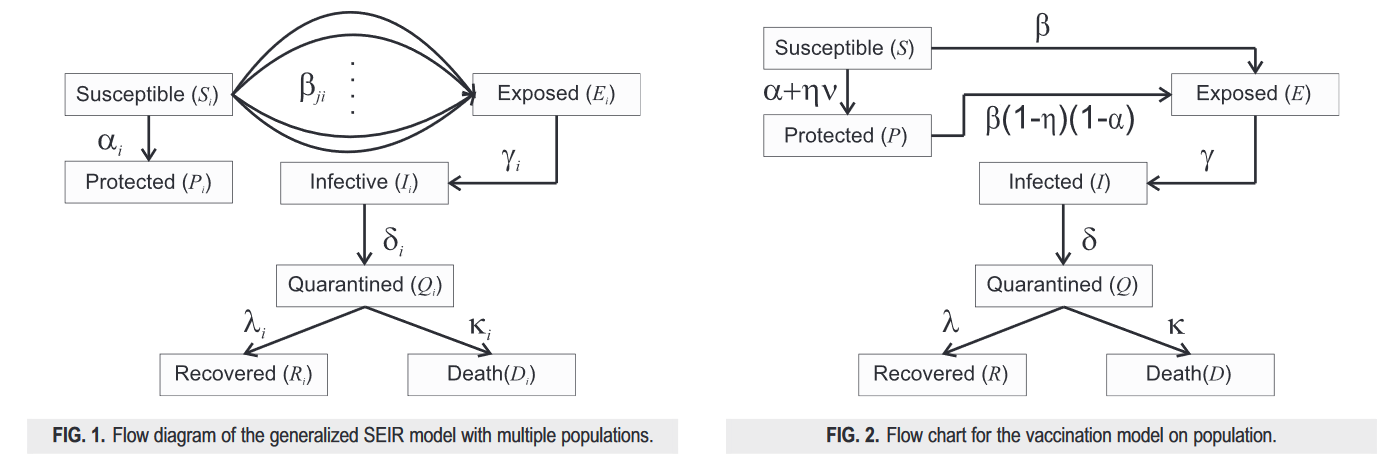
\includegraphics[width=10cm]{images/exchange-diagram-guino.png}%
		\caption{Diagrama de intercambio entre metapobalciones.}
\end{figure}

\begin{figure}[h!]
	\centering
		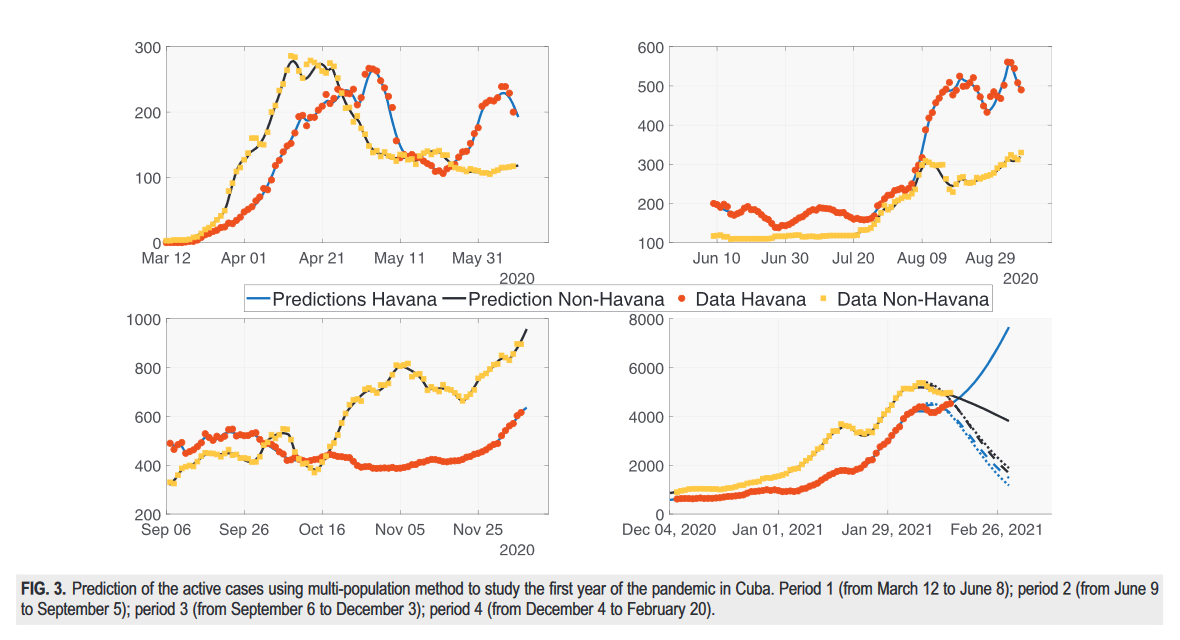
\includegraphics[width=10cm]{images/predictions-guino.png}%
		\caption{Predicciones del estudio en las diferentes metapoblaciones.}
\end{figure}


El artículo \cite{li2022geographical} analiza la distribución geográfica y factores de influencia en los casos de
COVID-19 en China. Utiliza varios indicadores socioeconómicos y ambientales para modelar la
influencia de factores como construcción urbana, PIB y emisiones industriales en la cantidad de pacientes y fallecidos
por la enfermedad. El análisis de interacción muestra efectos complejos entre los factores y los resultados sugieren
estrategias de salud pública localizadas basadas en los impulsores específicos de cada ciudad.
En resumen, el estudio aplica análisis espacial para caracterizar la heterogeneidad en la propagación de COVID-19 e
informar respuestas pandémicas adaptadas.

\begin{figure}[h!]
	\centering
		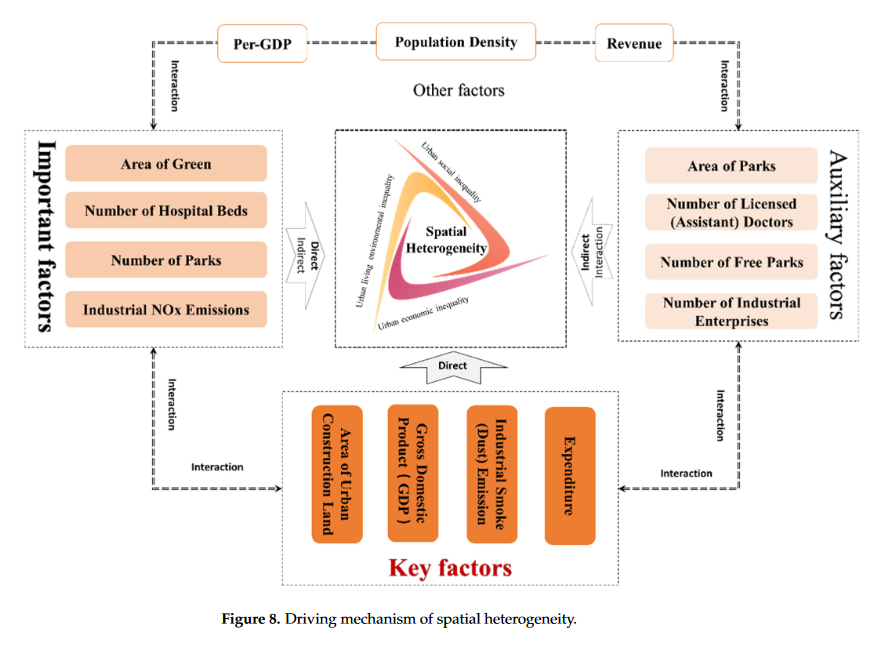
\includegraphics[width=10cm]{images/spatial-heterogenity-factos-weiwei.png}%
		\caption{Factores que influyen en la propagación y fallecimientos y cómo se relacionan los factores entre sí.}
\end{figure}

\section{Conclusiones}

Este reporte ha presentado una introducción a la Biomatemática y el uso de modelos para representar la
heterogeneidad espacial en sistemas biológicos. Se ha mostrado cómo la inclusión explícita del espacio en
modelos epidemiológicos y ecológicos puede mejorar nuestra comprensión de procesos complejos en el mundo real.

El curso me ha provisto de conocimientos valiosos sobre los principios de la modelación matemática en biología
y las técnicas para desarrollar modelos que capturen interacciones espacialmente explícitas. El uso de ejemplos
y aplicaciones a problemas actuales ha facilitado la comprensión de los conceptos teóricos.

Entre los principales aprendizajes se encuentran: los enfoques para representar espacialmente sistemas biológicos,
el esquema de modelado presentado, y ejemplos de modelos espacialmente explícitos como el SIR con movimiento y
modelos en redes. Estas herramientas me permitirán construir modelos más realistas de fenómenos ecológicos y
epidemiológicos.

\addcontentsline{toc}{section}{Introduction} % Adds this section to the table of contents



%\begin{figure}[h!]
%	\centering
%		\includegraphics[width=10cm]{}%
%		\caption{}
%\end{figure}








%----------------------------------------------------------------------------------------
%	REFERENCE LIST
%----------------------------------------------------------------------------------------
\phantomsection
\bibliographystyle{unsrt}
\bibliography{references}

%----------------------------------------------------------------------------------------

\end{document}